Currently Kubernetes implements horizontal pod auto-scaling.
As this title suggests, auto-scaling in
Kubernetes involves creating and deleting replica pods for a specific replication
controller such that the replicas handling the requests load-balanced by a service
operate within a specified resource range. A visual representation of this
process can be seen in Figure \ref{fig:kubernetes-visualization-with-autoscaler}.

Kubernetes implementation of auto-scaling is referred to as horizontal because
auto-scaling occurs by creating replicas of each pod and then dividing the work
among these replicas, as opposed to expanding the resources of any single pod.
While not yet implemented, Kubernetes reliance upon containers means vertical
auto-scaling is a possibility in the near future, as there are a variety of
methods for increasing the resources available to a container without stopping
execution \cite{docker-up-and-running}.

\begin{figure}[!h]
  \centerline{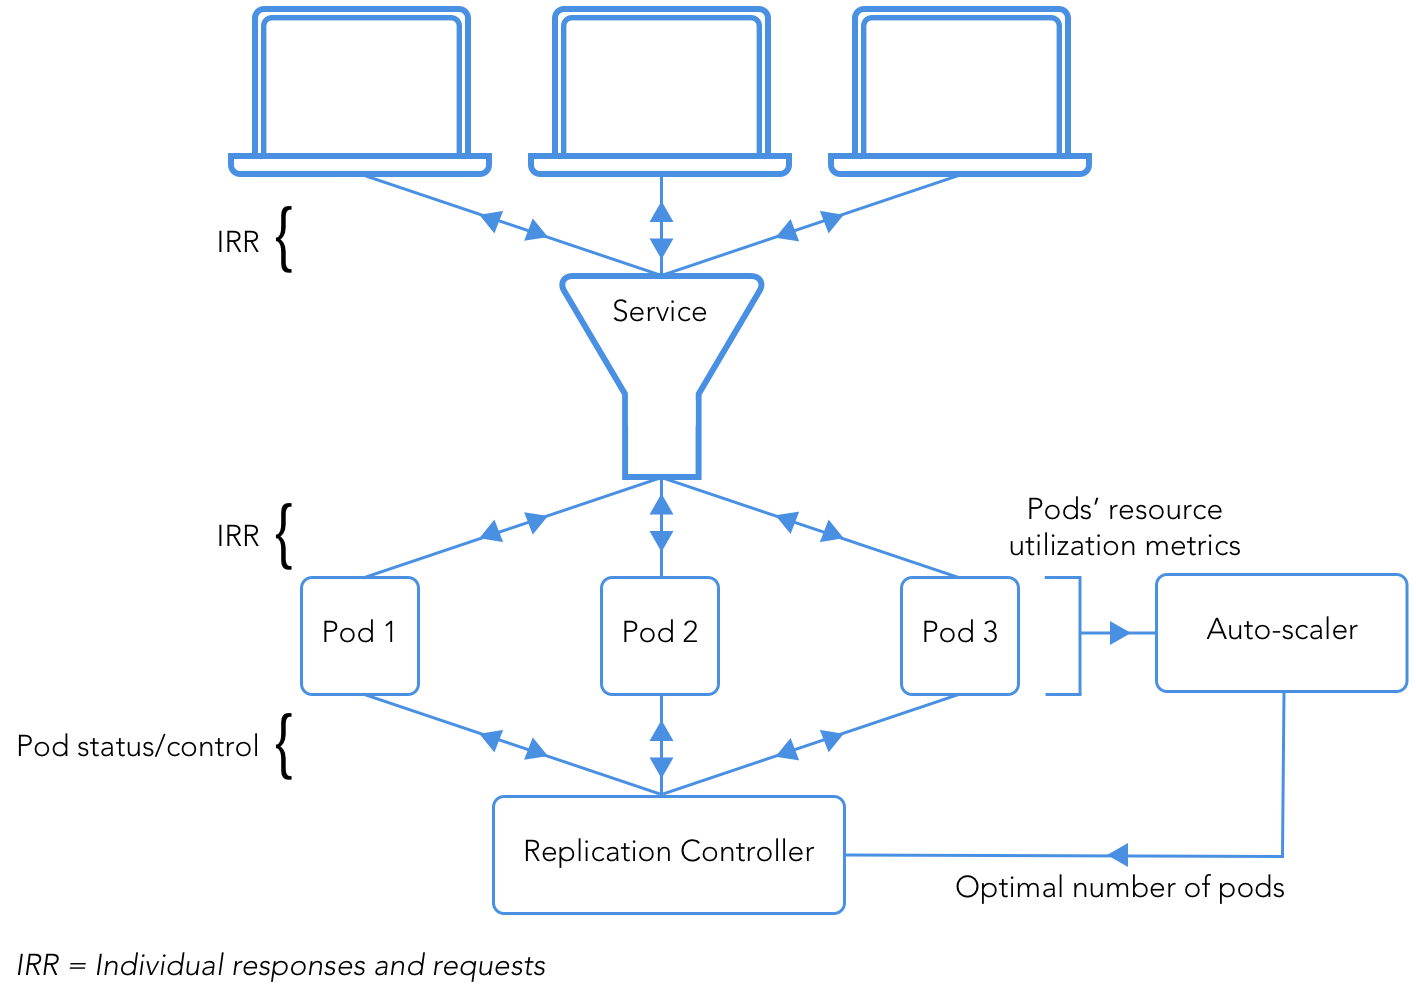
\includegraphics[scale=.25]{kubernetes-visualization-with-autoscaler.png}}
  \caption{A visualization of Kubernetes with autoscaler}
  \label{fig:kubernetes-visualization-with-autoscaler}
\end{figure}

As was distinguished in the background section, Kubernetes currently implements reactive
feedback control auto-scaling, which is when auto-scaling occurs to
ensure the preservation of a certain state.
In Kubernetes, the auto-scaler operates as a control loop,
as it queries pods at a set interval to determine
their current resource utilization, and performs auto-scaling actions to
preserve our desired level of per replica pod resource utilization.
At the start of this thesis, the only resource on which it is possible to
determine auto-scaling behavior is CPU utilization percentage, although since
then Kubernetes has added support for auto-scaling based on custom metrics such
as memory usage. Nonetheless, we focus on auto-scaling based on percentage CPU
utilization throughout this thesis.
Thus, based on the average CPU utilization percentage, the
auto-scaler will create or delete replica pods to ensure average CPU utilization
percentage is within the target range the user specified when creating the
auto-scaler. The algorithm for determining the correct number of replicas
will be discussed in detail in the next section. Finally,
in order to ensure auto-scaling is not attempted too frequently, once a
scale up or scale down happens, no more auto-scaling will occur for a constant
threshold interval. As of the implementation at the beginning of this thesis,
this interval is currently five minutes from the most recent
re-scaling for down-scaling and three minutes from the most recent re-scale for
up-scaling. This waiting time prevents thrashing by ensuring
auto-scaling can actually take effect before it is potentially attempted again
\cite{k8s-horizontal-pod-autoscaler-user-guide}.\footnote{We modify the length
of the forbidden window when running our predictive auto-scaling trials, as will
be discussed in Section \ref{autoscaling-predictively}.}
